\chapter{Modelling a bio-inspired series-viscoelastic actuator} \label{ch7:ModelingBio}

\section{Introduction}

In the previous chapters, the development of two modelling tools based on the LVMs, and one modelling tool based on machine learning algorithms is described. The three developed models are capable of accounting for the nonlinear velocity-dependent stress response of the studied soft materials with adequate accuracy. Due to the measurement of performance used for evaluating the ANN models, further validation is desired. Specifically, under a simulated real-time scenario, which replicates the conditions expected in a real robotic application. This is in line with the motivation of this research of addressing the current limitations of traditional modelling tools when being deployed as part of a control system, such as: high complexity and large computational power requirements.

In this chapter, the performance of the ANN model is assessed under a simulated real-time scenario. This is done by assessing the prediction performance of the ANN model under different types of strain inputs, such as a sine wave, and using a simplified model of a series-viscoelastic actuator. This study is performed in Simulink. The developed PL models are not included in this analysis due to their formulation which make use of past values of the stress response of the material. This contradicts the principles and benefits of series-elastic actuators.

Also included in this chapter is the investigation about the similarities between the human tendon and the studied soft materials. This is a crucial part for selecting the best soft material to be implemented as part of the model of a series-viscoelastic actuator. 

Results highlight an unexpected limitation of the developed ANN model which is not capable of performing well under a variable strain rate input. This can be circumvented by keeping the strain rate input constant. However, this is a limitation which must be addressed for the ANN model to be reliable in real robotics applications.

In summary, the design process presented in here consists of: the selection of the best soft material to match the human tendon properties; the selection of the electric motor and gearbox combination suitable to deliver 50\% assistance, based on the knee torque requirements during walking activities; the evaluation of the ANN model in simulated real-time under different strain input signals; and the 3D design of a clamping device aimed to hold several pieces of soft materials in a bundle-form.

\section{Matching the Human Tendon Properties}

In line with the aim of implementing the human skeletal muscle system functionality in soft robotic applications in the form of a bio-inspired soft actuator, this section presents a comparison analysis between the mechanical properties of the seven studied soft materials, and the human tendons and ligaments involved in the motion of the knee joint. The latter is motivated due to the large contribution of this joint on the activities of daily living, as described in \Cref{sec:chapterDesignGuidelines}. Due to the limited availability of clinical studies focusing on the tensile strength and stress relaxation properties of the tendons and ligaments involved in the human knee joint, a selection of three separate clinical studies is made. The first study is solely focused on the tensile strength properties of the patellar tendon \cite{johnson1994tensile}, the second one is focused on the stress relaxation properties of the quadriceps ligaments \cite{schatzmann1998effect}, and the third study is focused on the tensile strength properties of both the patellar tendon and the quadriceps ligaments \cite{staubli1999mechanical}. The aim of this comparison analysis is to identify which of the studied soft materials can match the human tendon mechanical properties. Due to this, the viscoelastic properties of the human patellar tendon and the quadriceps ligaments are compiled in \Cref{tbl:tendon&soft}, alongside the mechanical properties of the studied soft materials for direct comparison.

\begin{table}[htbp!]
    \centering
    \caption[Viscoelastic properties of the patellar tendon and the quadriceps ligament, compared against the viscoelastic properties of the studied soft materials (\Cref{tbl:stressRelProperties,tbl:elasticProp}).]{Viscoelastic properties of the patellar tendon and the quadriceps ligament \cite{johnson1994tensile,staubli1999mechanical,schatzmann1998effect}, compared against the viscoelastic properties of the studied soft materials (\Cref{tbl:stressRelProperties,tbl:elasticProp}).}
    \begin{tabular}{lcccccccc}
    \toprule
    & Human & EPR & FR & NatPolR & NR & PR & SR & NatR \\
    & Tendon \\
    \hline
	Tensile Strength \\
    \hline
    $\sigma_{ue}$ (MPa)     & 33.6   & 8.48 & 4.36  & 3.57  & 3.55  & 0.3   & 6.03  & 9.43  \\
    $\varepsilon_{ue}$      & 0.14   & 7.56 & 3.97  & 1.19  & 3.57  & 1.87  & 5.77  & 13.02  \\
    $E_{small}$ (MPa)   & 303.9  & 3.23 & 4.83  & 9.97  & 4.29  & 0.58  & 3.26  & 1.01  \\
    \midrule
	Stress Relaxation \\
    \hline
    $S.R$ (\%)                          & 41     & 32    & 67   & 35    & 29    & 63    & 31    & 15\\
    \bottomrule
    \end{tabular}
    \label{tbl:tendon&soft}
\end{table}

In \Cref{tbl:tendon&soft}, the large difference between the elastic properties of the quadriceps tendon and the studied soft materials, specifically for the elastic modulus $E_{small}$, can be appreciated. Nonetheless, the achieved stress relaxation in the human tendon is very similar to the one found in the soft materials. Therefore, they share similar viscous properties. This is a positive finding, because the elastic properties, of stress and strain, are structural parameters which depends on the dimensions of the material \Cref{sec:CharacterizationProcess}. The stress is inversely proportional to the cross-sectional area of the material. Moreover, the stress has a nonlinear relationship with the material strain. Hence, a material with larger cross-sectional area will require a larger force to achieve the same deformation. With this in mind, a new questioning arises regarding the cross-sectional area increment required for the soft materials to match the properties of the human tendon.

The latter questions must be answered considering the end application of the soft materials. As previously mentioned, these are intended to be used as part of a series-viscoelastic actuator. Having this in mind, the way in which the soft materials match the human tendon properties by an increase in their cross-sectional area can be better visualized. The implementation of a bundle of many strips of a soft material is proposed. The dimensions of each strip must be in line with the dimensions in which the material is available from the manufacturer. As previously mentioned, they all come in a rectangular shape. The thickness among all the studies soft materials vary from one to the other. Moreover, it is useful to think in the end application of the soft actuator itself, which is human assistance. According to the literature, a robotic wearable device for rehabilitation applications must deliver an assistance of 60\% of the peak torque required \cite{dos2014impedance}. Due to this, an objective assistance percentage of 50\% is proposed in here as design guidelines for the selection of the motor-gearbox combination. In addition to this, the safe working conditions of the studied soft materials, i.e. the elastic region, are considered. The approximated elastic region of each studied, using the offset-yield strength, is compiled in \Cref{sec:CharacterizationProcess}. Lastly, all this information is considered in the matching factor calculation, in which the elastic modulus $E_{small}$ of the human tendon is desired to be matched by the soft materials.

\begin{table}[htbp!]
    \centering
    \caption{Matching factors required for the soft materials to achieve the human tendon $E_{small}$ value. The width proposed for the material strips is 66 mm.}
    \begin{tabular}{lccccccc}
    \toprule
                            & EPR & FR & NatPolR & NR & PR & SR & NatR \\
    \hline
    Matching factors \\
    \hline
    $A_o$                   & 7 & 7 & 7 & 7 & 2 & 7 & 12\\
    $E_{small}$              & 77                     & 52           & 25                     & 58      & 375          & 76       & 248           \\
    $E_{small}$ @ 50\%                          & 39                     & 26           & 12                     & 29      & 188          & 38       & 124           \\
    \hline
    Material Dimensions \\
    \midrule
    Old $A_o$ $(mm^2)$              & 9 & 9 & 9 & 9 & 36    & 9 & 5.22  \\
    New $A_o$ $(mm^2)$         & 4852                   & 3245         & 1572                   & 3653    & 27020        & 4807     & 15517         \\
    New $A_o$ @ 50\% $(mm^2)$  & 2426                   & 1622         & 786                    & 1827    & 13510        & 2404     & 7758          \\
    Strip Width (mm)       & 66  & 66    & 66    & 66    & 66    & 66    & 66    \\
    No. of strips          & 49    & 33    & 16    & 37    & 68    & 49   & 270  \\
    No. of strips @ 50\%   & 25    & 16    & 8     & 18    & 34    & 24   & 135  \\
    \bottomrule
    \end{tabular}
    \label{tbl:matching}
\end{table}

The matching factors described in \Cref{tbl:matching} are obtained using a two-fold process. Firstly, the cross-sectional area of each soft material is matched with the cross-sectional area of the human tendon. Secondly, the elastic modulus of the human tendon is matched, considering the previous increase in the cross-sectional area of the materials. As previously mentioned, the materials thickness is defined by the manufacturer, therefore fixed. Nonetheless, many strips can be extracted from the material rectangular sheet using laser cutting. The width of these strips can be modified to increase the cross-sectional area of the material. Hence, a width of 66 mm is proposed for the latter calculations. The latter is decided taking into consideration the application in which the bundle of strips will be implemented. That is, bio-inspired actuator. Moreover, this actuator is aimed to be used to assist the knee joint. This in fact puts a limit to the width of the bundle of strips, and that is the dimensions of the human shank. Taking this into consideration, and the relationships between the required number of strips and the strips width. The previously mentioned value of 66 mm is adequate. In theory, it is possible for all the materials to match the human tendon elastic modulus as long as enough strips are used. The exact number is stated in \Cref{tbl:matching}. Finally, by analysing the obtained matching factor in combination with the stress relaxation properties of the human tendon, the soft material with the closest properties is identified to be the NatPolR material.

\section{Validation in Simulated Real-time}

In this validation, the developed PL models are not included because its formulation makes use of past values of the stress response. This contradicts the benefits of implementing a SEA in the first place, which is to use the deformation of the elastic element as an indirect way to measure the stress response. The same principle apply for series-viscoelastic actuators (SVAs). 

The developed ANN models, takes two inputs, the strain and strain rate, and outputs the stress response of the material in MPa. Therefore, particular care must be taken with regard to the conversion to avoid undesired results. As previously mentioned the stress is defined as $\sigma = F/A_o$, whereas the strain is defined as $\varepsilon = \Delta L / lo$. The value of $lo=33mm$ applies to all soft materials studied in here. The cross-sectional area $A_o$ varies from one material to the other. The units from the stress output (MPa) and $A_o$ ($mm^2$) are compatible and can be used as they are in the conversion. 

The simulation environment is based on the model of a soft SVAs. Commonly, these actuators are cable-driven. In simple terms, this means that an electric motor is connected in series to a viscoelastic element, and this element to a load. In here, many assumptions are make to simplify the model of the actuator and isolate the performance of the ANN model. These assumptions are as follows:

\begin{itemize}
	\item The electric motor is replaced with a simple sine wave block which represents the strain. The derivative of this input signal is the strain rate.	
	\item The viscoelastic element is connected to the motor in one end, and is fixed on the other end. Hence, no load is connected to this element.
	\item The concept of implemented multiple pieces of the same material is implemented by a gain block.
\end{itemize}

Having defined the conditions of the simulation, the developed Simulink model is illustrated in \Cref{fig:ANNStepTest}, as follows:

\begin{figure}[hbtp!]
    \centering
    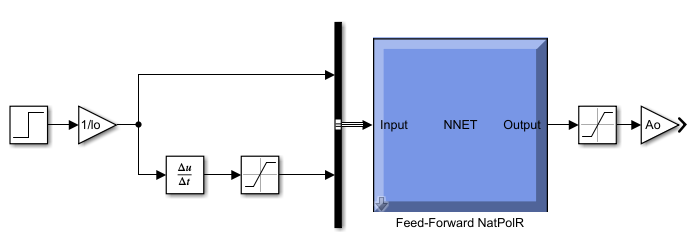
\includegraphics[width=\textwidth]{ANNStepTest.png}
    \caption{ Simulink implementation of the ANN model. The ANN model takes the strain and strain rate as inputs, and delivers the stress response of the material in MPa as output. The gain blocks ensure that the units are consistent. }
    \label{fig:ANNStepTest}
\end{figure}

\newpage

In \Cref{tbl:matching}, the NatPolR material is identified as the best candidate to imitate the mechanical properties of the human tendon. Due to this, the NatPolR material is selected for this simulation. The parameters of the generated sine wave must be inside the working conditions of this soft material. The latter is reported in \Cref{tbl:elasticProp}. The elastic limit $\varepsilon_y$ of the NatPolR varies from  0.41 to 0.48 strain. Similarly, the stress response of the material in this range of deformation goes from 2.12 to 2.52 MPa. Moreover, the prediction capabilities of the ANN models have been assessed for the three available strain rates of 50, 250, 500 mm/min. Therefore, the frequencies of the generated sine wave must be inside this range as well. For consistency, these values are changed to mm/sec when defining the sine wave. Inside the block diagram, the generated sine wave is divided by the initial length of the material $l_o = 33 mm$, yielding the units of the strain (mm/mm) per second. The generated sine wave must have positive values of the strain only. This is in line to the training set where only positive values of the strain are available. The generated sine waves follow the basic formula $f(t) = A sin(wt+\beta) + C$. For simplicity, only the amplitude $A$ and the offset $C$ are varied. Changing these two parameters allows each sine wave to have different values of strain rates, measured as the difference between the maximum and minimum values of the sine wave that are spaced by one second due to the chosen frequency.

A total of four different sine waves are generated to represent a varying strain inputs. The strain rate input is the derivative of the sine wave, i.e. a cosine wave. Each one is aimed to assess a specific scenario. The sinewaves with the strain rate of 100 mm/min and 400 mm/min are aimed to assess the response of the model for positive values of the strain and the strain rates which are unknown to the ANN model, i.e. they are not included in the training set. The sinewave with a strain rate of 50 mm/min is aimed to assess the response of the ANN model when negative values of both the strain and strain rate are included. In reality, negative values of the strain, i.e. compressing the material, do not produce any stress response. Nevertheless, this behaviour must considered when deploying the ANN model in a control system. Lastly, the sine wave with a strain rate of 500 mm/min is aimed to assess the response of the ANN model when the strain rate is saturated, i.e. negative values of the strain rate are replaced with zero. The results of the simulation are illustrated in \Cref{fig:ANNSineTest}.

\begin{figure}[htb!]
	\centering
	\begin{subfigure}[b]{0.49\textwidth}
		\centering
		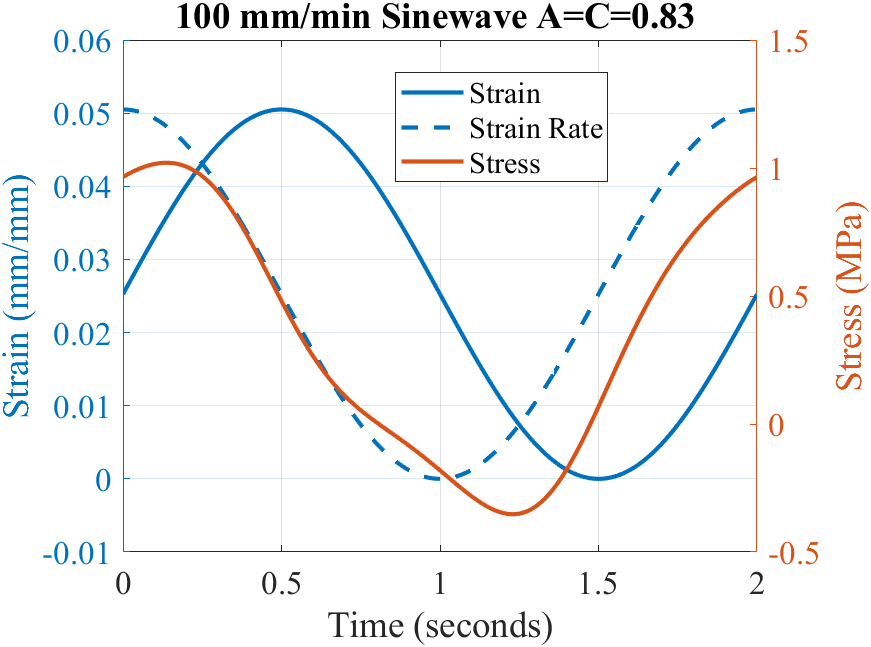
\includegraphics[width=\textwidth]{Sinewave100.png}
		\caption{}
		\label{fig:ANNSineTesta}
	\end{subfigure}
	\begin{subfigure}[b]{0.49\textwidth}
		\centering
		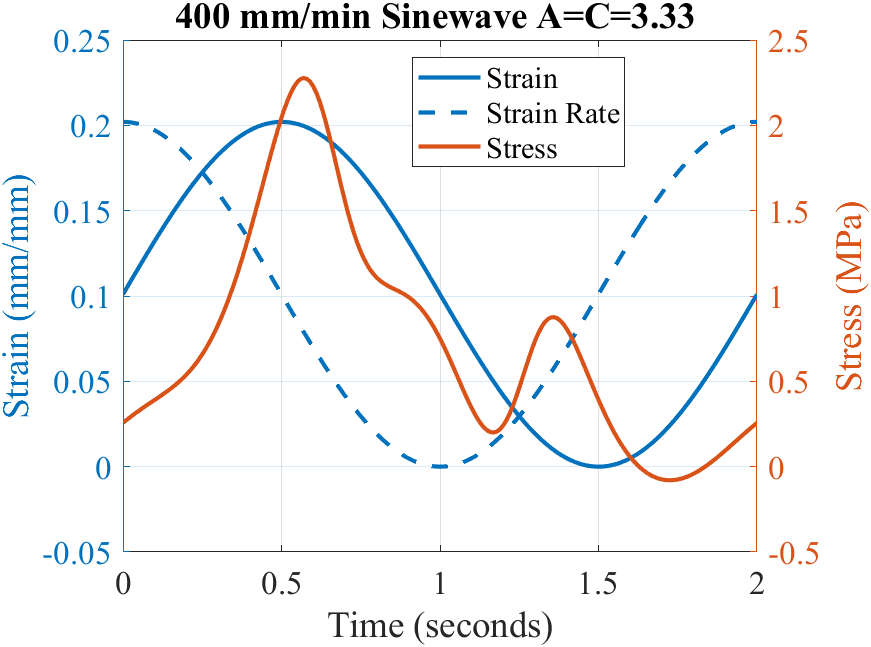
\includegraphics[width=\textwidth]{Sinewave400.png}
		\caption{}
		\label{fig:ANNSineTestb}
	\end{subfigure}
	\begin{subfigure}[b]{0.49\textwidth}
		\centering
		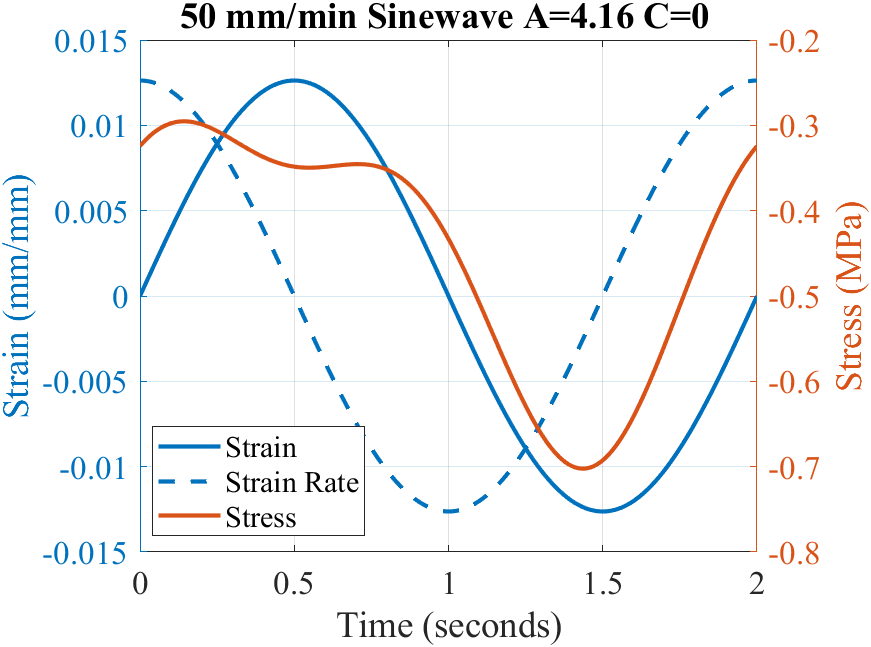
\includegraphics[width=\textwidth]{Sinewave50.png}
		\caption{}
		\label{fig:ANNSineTestc}
	\end{subfigure}
	\begin{subfigure}[b]{0.49\textwidth}
		\centering
		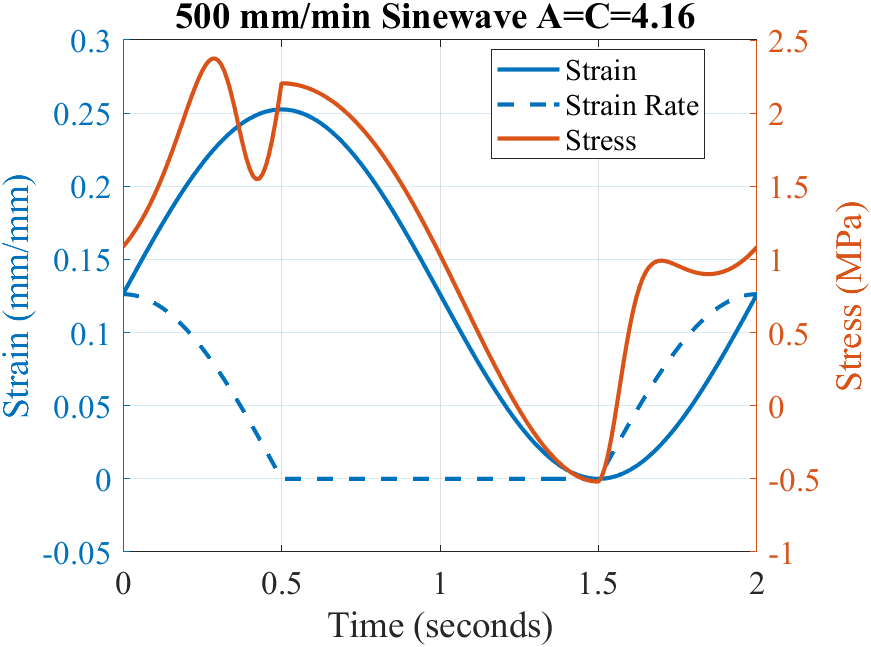
\includegraphics[width=\textwidth]{Sinewave500.png}
		\caption{}
		\label{fig:ANNSineTestd}
	\end{subfigure}
	\caption{ANN model stress response to a sine wave strain input. The solid and dotted blue line are the strain and strain rate, respectively. (a) and (b) positive and unknown strain rate values, (c) negative values of the strain and strain rate, (d) strain rate saturated to avoid negative values.}
	\label{fig:ANNSineTest}
\end{figure}

The prediction of the ANN model under scenario (a) is not entirely accurate since negative values of the stress response are present (\Cref{fig:ANNSineTesta}). This is an unexpected behaviour because both the strain and strain rate are positive and are inside the elastic limit of the material. This behaviour can be caused by the steep decaying rate of the cosine wave in the 0.5 to 1.5 seconds interval. Nonetheless, the stress response of the ANN model is even more unstable when using a larger value for the strain and strain rate as shown in scenario (b) (\Cref{fig:ANNSineTestb}). In here, the response of the ANN model do not reach negative values. In scenario (c), the response of the model looks very stable. However, the stress response is always negative (\Cref{fig:ANNSineTestc}). This scenario is initially out of the ordinary due to the negative values of the strain and strain rate which are not expected to be present in a real application. Due to this, the obtained stress response if expected to be inaccurate. Lastly, in scenario (d) the response of the ANN model oscillates between positive and negative values despite the saturation implemented to the strain rate signal (\Cref{fig:ANNSineTestd}). In summary, the scenario in which the ANN model performed the best is in (a). Although, the obtained negative values of the stress response are undesired.

The unstable response of the ANN model can be caused by the limited number of strain rates included in the training set.  Moreover, the strain rate in these scenario is changing over time, whereas the strain rate in the training set is fixed between three different values. Due to this, the four scenarios are tested again, this time using a positive an constant strain rate of 250 mm/min. The results are illustrated in \Cref{fig:ANNSineCTest}.

\begin{figure}[htb!]
	\centering
	\begin{subfigure}[b]{0.49\textwidth}
		\centering
		\includegraphics[width=\textwidth]{Sinewave100C.png}
		\caption{}
		\label{fig:ANNSineCTesta}
	\end{subfigure}
	\begin{subfigure}[b]{0.49\textwidth}
		\centering
		\includegraphics[width=\textwidth]{Sinewave400C.png}
		\caption{}
		\label{fig:ANNSineCTestb}
	\end{subfigure}
	\begin{subfigure}[b]{0.49\textwidth}
		\centering
		\includegraphics[width=\textwidth]{Sinewave50C.png}
		\caption{}
		\label{fig:ANNSineCTestc}
	\end{subfigure}	
	\caption{ANN model stress response to a sine wave strain input and a constant strain rate. The solid and dotted blue line are the strain and strain rate, respectively. (a-b) positive and unknown strain values, (c) negative values of the strain.}
	\label{fig:ANNSineCTest}
\end{figure}

The response of the ANN model when a constant strain rate is used is very stable (\Cref{fig:ANNSineCTest}). This further indicates that the main limitation of the developed ANN models, i.e. their performance relies heavily on the training set. This can be improved by adding the unloading stage of the stress-strain curve of the material. In this way, the concept of a decreasing strain rate can be learned by the ANN model. 

Summarizing, the analysis performed in this section provided useful information about the behaviour of the ANN model in simulated real-time conditions. An important limitation is found, which is the erratic prediction of the ANN model when the strain rate varies over time. The lack of a bigger and richer training set is identified as the potential cause. The relevance of understanding the role of the strain rate on the stress response of soft materials has been recently highlighted in the literature. In the work performed by Xu t al. in 2019, the development of an ANN model capable of predicting the elastic modulus of soft materials under different strain rates is described \cite{xu2019artificial}. The studied material in this case is a graphene reinforced composite, and is characterized using a dynamic mechanical analysis over a range of frequencies and temperatures. These ranges of values are the input of the ANN model which in fact, does not directly predict the stress response of the material, and instead, predicts the storage modulus of the material which is a parameter related to the viscoelasticity of materials. Using this parameter in combination with known mathematical equations, the stress response of the material can be extracted. Ongoing research about the modelling of soft materials using ANN models highlights the relevance and feasibility of the research presented in this thesis.

\section{Series-viscoelastic Actuator: Design Concept }

Series and parallel elastic actuators have been implemented in human assistance applications to achieve a muscle-like performance and increase the assistance capability of robotic wearable devices. Traditionally, the mechanical element used to provide elasticity in actuators is a metallic spring. However, the idea of replacing the metallic spring with a soft material, such as rubber, is being researched now. The works performed by D. Rollinson has proved this idea to be beneficial for series-elastic actuators (SEAs) by developing a rotational spring based on natural rubber \cite{rollinson2013design,rollinson2014design}. In fact, the latter research gave birth to HEBI Robotics and to the first SEA implementing a soft material as the elastic element \cite{HEBI2019}. In addition to this, other SEA concepts implementing rubber \cite{austin2015control}, dielectric elastomer \cite{bolivar2016towards} and polyurethane \cite{martins2015polyurethane} are being researched.

The benefits of series and parallel elasticity have been demonstrated in many works both with rigid and soft materials as the elastic element. However, there is only one actuator concept documented in the literature which implements both series and parallel elasticity in the same actuator, creating a series-parallel-elastic actuator (SPEA) \cite{mathijssen2014variable}. This actuator implements rigid springs and is based on the variable recruitment process observed in human muscles, which means that depending on the required torque and displacement, more springs are engaged.

As previously mentioned, an objective assistance of 50\% of the required peak torque is proposed. Moreover, the research is focused on the human knee joint due to its major role in the activities of daily living. In line with this, the required peak torque and angular speed range for the knee joint during normal walking is found to be 29 Nm and $\pm$50 rpm respectively \cite{dos2014impedance,winter2009biomechanics}. Therefore, the peak torque aimed to be delivered to achieve a 50\% assistance is 15 Nm. The previous parameters will be used as guidelines when selecting the electric motor/gearbox combination to be used in the simulation. In addition to this, the working range of the soft materials is also important. The latter is indicated by the elastic region of the material, which is approximated using the offset yield strength in \Cref{sec:CharacterizationProcess}. In summary, the parameters aimed to be used in a future experimental validation are presented in \Cref{tbl:simParameters}.

\begin{table}[hbt!]
    \centering
    \caption{Simulation parameters}
    \begin{tabular}{ll}
    \toprule
    Soft Material       & Natural Rubber with Polyester (NatPolR)\\
    Working Range       & Up to 0.5 strain ( 16.5 mm)\\
    Strip Width        & 20 mm\\
    Strip length       & 33 mm\\
    $A_o$               & 9 $mm^2$\\
    No. of strips      & 8\\ 
    Torque reference    & Knee joint motion capture data \\
    Position reference  & Knee joint motion capture data \\
    \midrule
    Electric motor      & Maxon RE53-323891 \cite{Maxon2019motor}\\
    Nominal Voltage     & 24 V\\
    $L_a$               & 0.191 mH\\
    $R_a$               & 0.583 $\Omega$\\
    $K_a$               & 29.2 mNm/A\\
    $K_b$               & 0.029 V/(rad/s)\\
    $J_m$               & 79.2 g/$cm^2$\\
    \midrule
    Gearbox             & Maxon GP 42 C-203124 \cite{Maxon2019gearhead}\\
    $n$                 & 1/81\\
    \end{tabular}
    \label{tbl:simParameters}
\end{table}

As part of the preliminary design of the series-viscoelastic actuator, and in line with using a bundle of soft materials to match the human tendon mechanical properties, a clamping device is designed in SolidWorks\textregistered{} (\Cref{fig:ClampWhole}). The width of the clamp is in line with the end application, which is an assistive wearable device for the human knee joint. The idea behind this design is to stack several pieces of the same material on top of each other and then clamp them together to create a bundle of soft materials. This design is similar to the one used in the literature when dealing with rubber materials and cable-driven actuators \cite{austin2015control}.

\begin{figure}[htb!]
	\centering
    \begin{subfigure}[b]{0.49\textwidth}
        \centering
        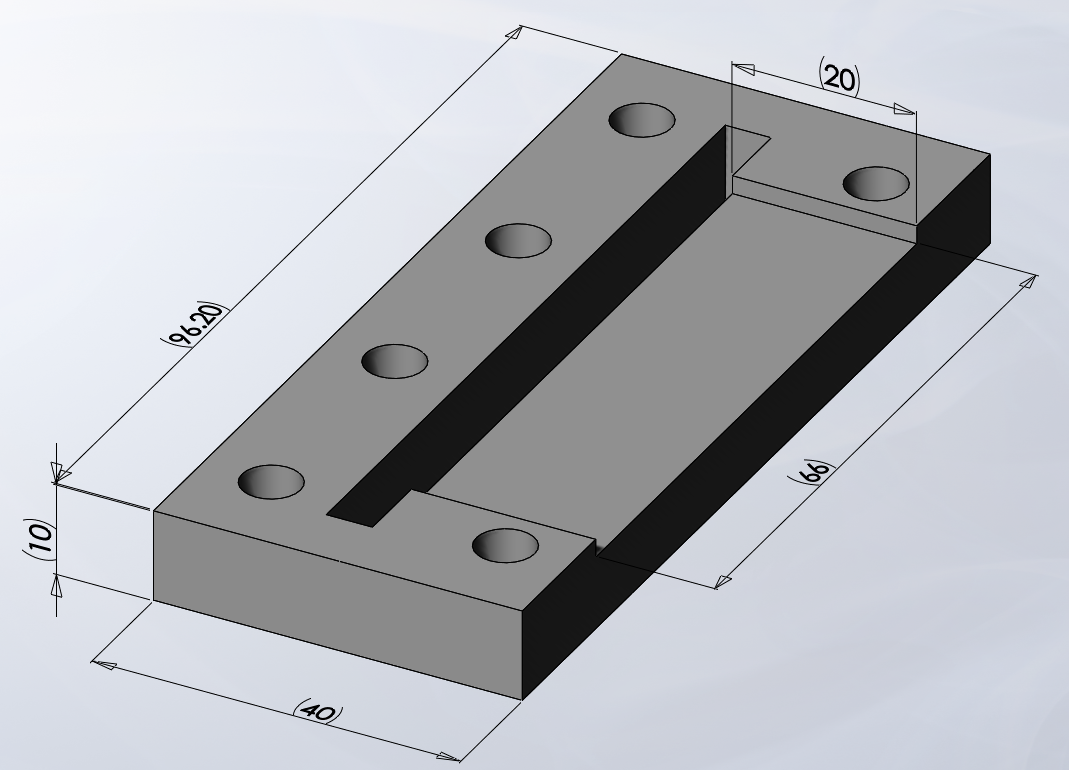
\includegraphics[width=\textwidth]{ClampBase.PNG}
        \caption{}
        \label{fig:ClampBase}
    \end{subfigure}
    \begin{subfigure}[b]{0.49\textwidth}
        \centering
        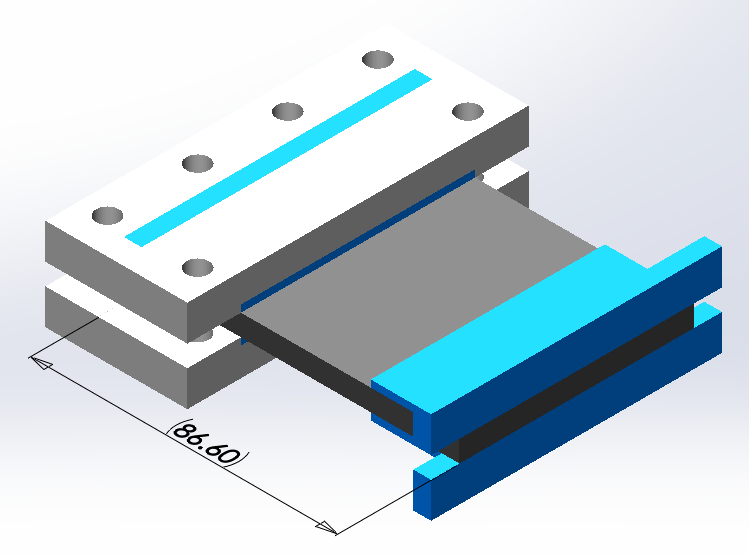
\includegraphics[width=\textwidth]{ClampedElement.PNG}
        \caption{}
        \label{fig:ClampElement}
    \end{subfigure}
    \caption{CAD Design of the detachable clamping device (a) Bottom part, (b) Final assembly, the soft material is coloured in black, and the T-shape attachment in blue. Units are in millimetres.}
    \label{fig:ClampWhole}
\end{figure}

The clamp mechanism of \Cref{fig:ClampWhole} is designed to be detachable. This is achieved by having a T-shape element which can be glued to a bundle of materials strips. Each soft material strip must also be glued to each other to allow for even deformation of the whole bundle. The T-shape attachment, which resembles a ``plug and play'' device, fits inside the clamp base (\Cref{fig:ClampBase}) and also in the clamp top element. This allows the quick testing of different bundles of soft materials. Once in place, the clamp mechanism can be secured with bolts going through the holes added to the clamp base and top parts. This is illustrated in \Cref{fig:ClampElement}. This design is inspired in the one used in \cite{austin2015control}, with the addition of designing it as detachable clamping mechanism to allow the test of different soft materials bundles, when being used as part of a test bench.

\section{Summary}

In this chapter, the preliminary design concept of a series-viscoelastic actuator is presented. As the very first step in the design process and in line with the aim of mimicking the human muscle skeletal system, the comparison of the human tendon mechanical properties against the properties of the soft materials is made. In addition to this, the validation of the ANN model performance under simulated real-time conditions is investigated. The results are unexpected due to the erratic stress response prediction of the ANN model. The latter is directly related with the fact that only up to three different strain rates are included in the training set. Moreover, the stress response of the ANN model is also affected by the selection of frequency and amplitude of the strain input. Nonetheless, the prediction performance of the ANN model is very stable when the strain rate is positive and constant. This highlight the necessity of a richer dataset which includes the unloading stage of the stress-strain curve of the materials. Also, information about a decreasing strain rate can improve the performance of the ANN model described in here. Finally, the work related to the design process of the series-viscoelastic actuator is presented, which includes: the selection of actuator technologies, selection of the best soft material to match the human tendon properties, and design of a clamping device to hold a bundle of stacked soft material pieces.